\section{Task 2}

\subsection*{Research object:}

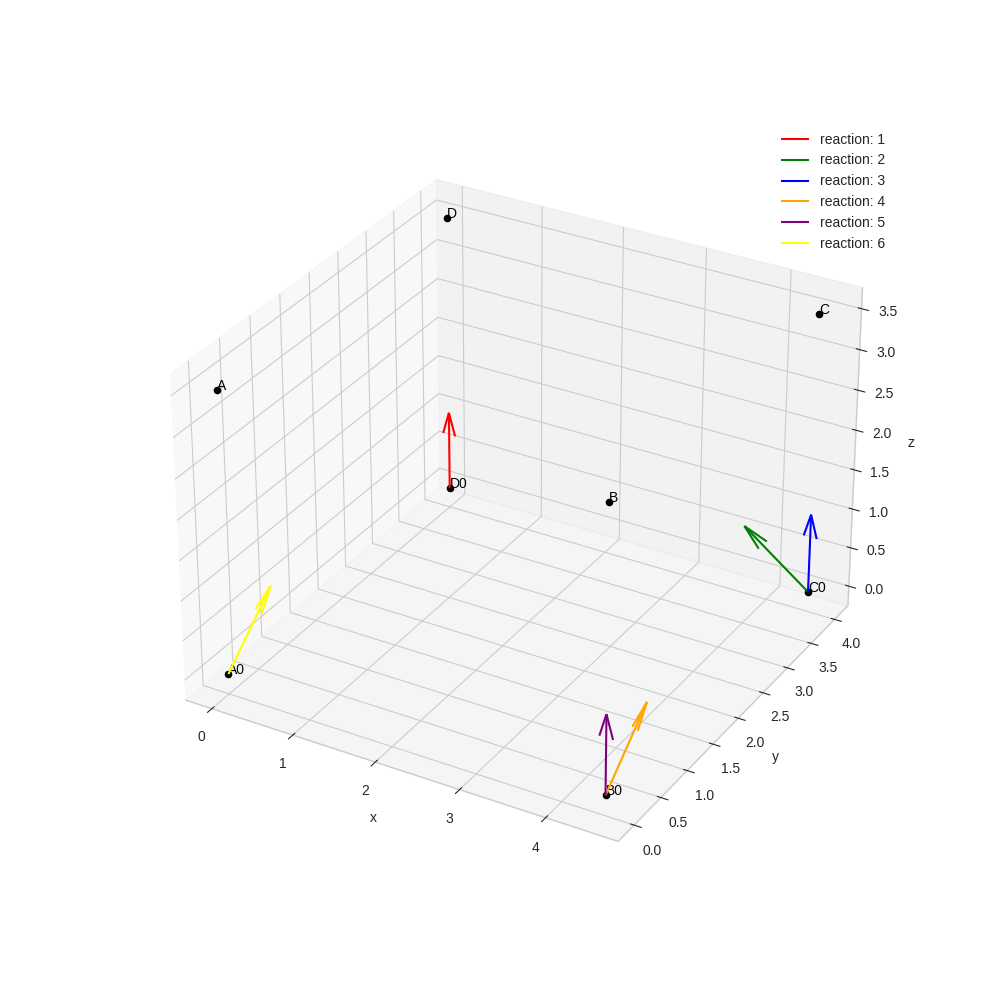
\includegraphics[width=\linewidth]{task2init.png}

\begin{enumerate}
    \item One rigid body $ABCD$ - plate
    \item $A_0A$, $B_0B$, $C_0C$, $D_0D$ - rods supporting the plate
    \item $A_0$, $B_0$, $C_0$, $D_0$ - hinge supports - $R_{ix}, R_{iy}, R_{iz}$
\end{enumerate}

\subsection*{Force analysis:}

\begin{enumerate}
    \item Rods will have reaction force codirected with the rod
    \item Thus, we have 6 forces: $\vec{R}_i, i \in [0, 5]$ to determine.
    \item $\vec{G}$ - gravitational force (given)
    \item $\vec{P}$ - action force (given)
\end{enumerate}

\subsection*{Solution:}

\begin{enumerate}
    \item We have to construct 2 equations because body should be static
          in terms of forces and moments.
    \item Forces equilibrium:
          \begin{align}
              \sum_{i=0}^5 \vec{R}_i + \vec{G} + \vec{P}= 0
          \end{align}
    \item Let $\vec{r}_i, i \in [0, 5]$ be vector from $A$ perpendicular to the force.
    \item Moments equilibrium:
          \begin{align}
              \sum_{i=0}^5 \vec{r}_i \times \vec{R}_i + \begin{bmatrix}
                  b/2 \\ a/2 \\ 0
              \end{bmatrix} \times \vec{G} = 0
          \end{align}
    \item We have 6 equations and 6 unknowns, so we can solve the system.
\end{enumerate}

\subsection*{Answer:}

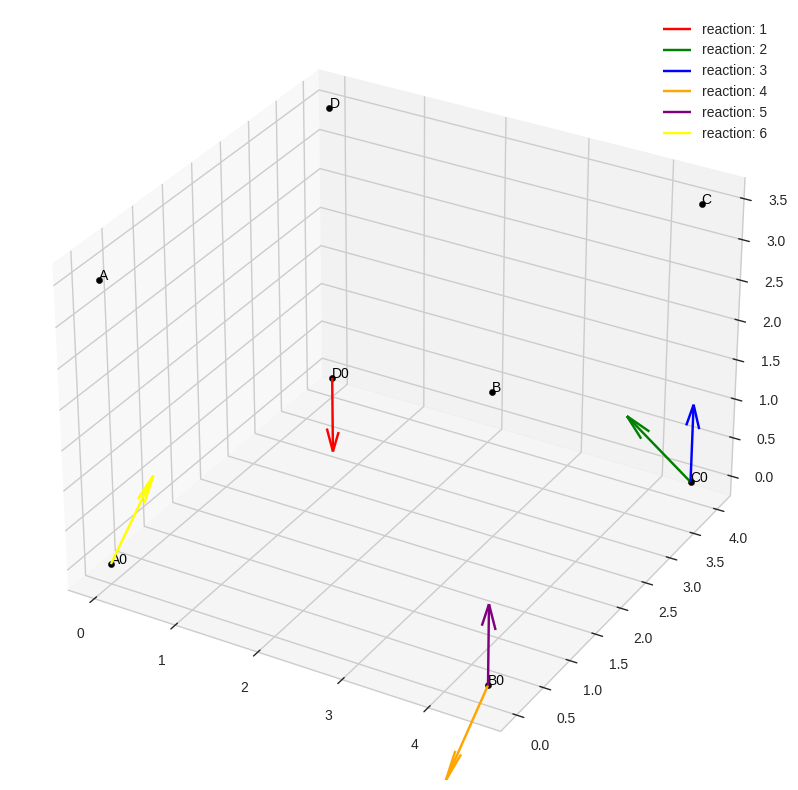
\includegraphics[width=\linewidth]{task2.png}

Image has already correct directions of reactions. Negative sign in the answer
means that the force is directed from top end of rod to its beginning. 
Shown reactions are only unit vectors for conviniency.

Obtained using python:

% [-37.66666667,  38.0058475 ,  23.33333333, -35.43381938,
% 9.        ,  35.43381938]

\begin{answer}
    \begin{enumerate}
        \item $R_1$ = $-37.66$
        \item $R_2$ = $38.01$
        \item $R_3$ = $23.33$
        \item $R_4$ = $-35.43$
        \item $R_5$ = $9$
        \item $R_6$ = $35.43$
    \end{enumerate}
\end{answer}
% \begin{enumerate}
% \end{enumerate}